\chapter{The algorithm}\label{cap:Algorithm}
We present here the algorithm we developed for data association with bearing only sensor.

The program takes as input a file that has a line for each step of the trajectory.
Each line specifies:
• The rototranslation with respect to the previous step (x, y, theta)
• a list of the measurements acquired in this step.

The basic idea is that, at each step, the algorithm iterates over all the observations associated with the considered position and tries to associate them with observations from the previous step, determining if each observation should be \textbf{queued} to one of the previous tracks or it should be associated to a new landmark.

A landmark is considered \textbf{confirmed} when it has at least a certain number of associated observations.

The \textit{track}, to which we will often refer in this chapter, is actually a landmark. When new observations are added to the track, the landmark position is re-estimated and the track is propagated to the next step.
When, on the contrary, no new observations are associated to the track, it is not propagated, and the landmark itself is either pruned or kept (depending on the fact that it had been confirmed or not).

Going on with the trajectory, the algorithm creates a graph, putting in it new poses and landmarks.

Every time a certain number of steps has been performed, the graph is optimized according to the edges created up to now.

After the trajectory evaluation is terminated, the optimized poses can be used to re-initialize the algorithm, keeping the bearing measurements unchanged, so to re-associate the data. This is known as \textit{Expectation Maximization}.

In section \ref{sec:issues} we illustrate the problems we had to face, and how we dealt with them.
After that, in section \ref{sec:pseudocode} there is a pseudo-code of the developed algorithm.

\section{Issues}\label{sec:issues}
\subsection{The main problem: vague observations}
Using a bearing only sensor involves a big problem: an observation is not enough to estimate the position of a landmark.
From an observation associated with a robot position we can only determine a line (actually an half line) where the landmark may be.
This is a problem because next step observations can't rely on the estimated position of the landmark for determining correspondances.

The developed algorithm deals with this problem distinguishing two cases (see figure \ref{fig:observation_association}):
\begin{enumerate}
  \item The landmark already has an estimated position.
  \item A position has not been estimated for the landmark. (Usually happens when the landmark has been seen only once)
\end{enumerate}
\begin{figure}[htbp]
  \centering
    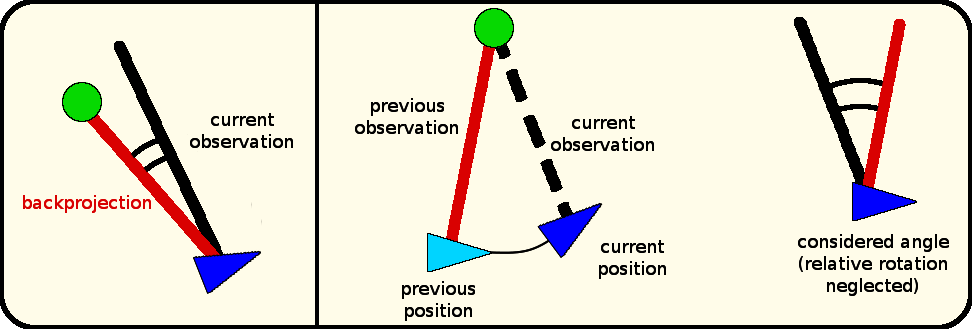
\includegraphics[width=0.8\textwidth]{images/observation_association.png}
  \caption{The two possible situations. The drawn angles are those to be evaluated.}
  \label{fig:observation_association}
\end{figure}
In the first case, the estimated position is backprojected on the robot pose, and the resulting angle is compared to the current observations.

In the second case, an assumption is made: given that the captures are ``close'', the sensed bearing for the same landmark should have remained similar between two consecutive steps. The comparation is then done only with the previous angle (of course after considering positions relative rotation).

\subsection{More than a close track}\label{subsec:twotracks}
It can happen that the observation we are evaluating is close to two of the tracks. There is of course a track that is ``closer'' than the other, but they are both inside a certain threshold.\footnote{We actually defined a threshold for the closer and another threshold for the second closer.}
In this case, we simply ignore the new observation.

\begin{figure}[htbp]
  \centering
    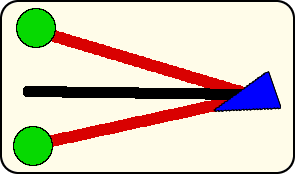
\includegraphics[width=0.3\textwidth]{images/uncertainty1.png}
  \caption{Two close observations. How to choose?}
  \label{fig:uncertainty1}
\end{figure}

To understand the sense of this choice, it is the case to highlight the importance of avoiding wrong associations.
Since we can only rely on the bearing for the landmarks position estimation, a wrong association can cause the graph to explode when optimizing.
This is then wiser, where possible, to avoid every source of uncertainty.
A pessimistic approach will possibly discard some good informations, but will be more reliable.

\subsection{Two observations for the same track}\label{subsec:twoobservations}
In section \ref{subsec:twotracks} we have seen that an observation could be close to two tracks.
We now face the dual problem: it can happen that two of the current observations are close to the same track.

\begin{figure}[htbp]
  \centering
    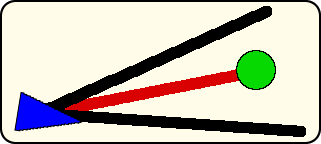
\includegraphics[width=0.3\textwidth]{images/uncertainty2.png}
  \caption{Two new observations are both close to the same track.}
  \label{fig:uncertainty2}
\end{figure}

Just like before, we cannot risk to associate a landmark with wrong measurements.
Moreover, it is obvious that a single landmark shouldn't generate two measurements.
Following the idea that not knowing is better than thinking wrong, we don't add either of the two observation to the track.
Anyway, the track is propagated to the next trajectory step.

\subsection{Further robustness}
Even with the precautions explained in sections \ref{subsec:twotracks} and \ref{subsec:twoobservations}, it can still happen that a wrong association is generated. In order to deal with this problem, the effect of edges in the optimization steps is limited via the use of the so called \textit{robust kernels}.
These are filters that impose a saturation threshold, over which the constraint effect can't grow anymore.
In chapter \ref{cap:Conclusions} we will see how this can enhance the results quality.

\section{Pseudo-code}\label{sec:pseudocode}
In this section, a pseudo-code for the algorithm is given.

First of all, some pseudo-structures.
\begin{itemize}
  \item RobotPosition: this represents a pose, and will contain:
    \begin{itemize}
      \item Coordinates and orientation (x,y,theta).
      \item A set of Observations.
    \end{itemize}
  \item Observation: this represents a measurement. It will be defined by:
    \begin{itemize}
      \item A reference RobotPosition.
      \item A bearing value.
    \end{itemize}
  \item Landmark: this represents a landmark, and is also used to propagate tracks. It will consist of:
    \begin{itemize}
      \item Coordinates (x,y).
      \item A set of references to Observations (all the observations that have been associated to this landmark)
    \end{itemize}
\end{itemize}

And here is the algorithm:

{\footnotesize
  \lstset{language=C}
  \begin{lstlisting}[frame=shadowbox,breaklines]
    definitions:
    	OPTIMIZE_EVERY	// every time this number of steps has been performed, an optimization sequence is made
    
    global variables: 
    	landmarks_list	// list where landmarks are inserted
        graph	// the graph to be used for optimization
        
    // This function manages the algorithm iterations.
    // 'steps' is the sequence of steps, each with the relative transformation with respect to the previous step and a set of observations.
    algorithm_launcher(steps)
    {
      // 'previous_observations' and 'propagate_observations' are lists used to keep track step after step of the observed landmarks
      previous_observations = new empty Landmarks list;
      propagate_observations = new empty Landmarks list;
      
      int loop_count = 0;	// increases at every step, is set to 0 when optimization is performed
      
      for each step
        loop_count ++;
      	current_position = compute the new position appending the new step to the previous one;
        current_position.observations = step.observations;
        
        // the observations propagated from the previous step are moved to the specific list
        previous_observations = propagate_observations;
        clear propagate_observations;
        
        propagate_observations = tryToUnderstand(current_position, previous_observations);
        
        if loop_count > OPTIMIZE_EVERY
        	loop_count = 0;
                populate the graph with new landmarks nodes and edges;
                graph.optimize();
        
      // end of 'for each step'
      
      // last optimization
      populate the graph with new landmarks nodes and edges;
      graph.optimize();
      
      // expectation maximization
      in case it is needed/required_by_the_user
      	steps = compute relative transformations from the optimized positions;
        algorithm_launcher(steps)	// rerun the algorithm
    }
    
    
    // this is the actual data association function
    // returns a Landmark list containing the tracks to be propagated to the next step
    tryToUnderstand(current_pose, previous_observations)
    {
      // prepare structures
      double expected[propagate_observations.size()];	// an array of doubles with a value for each of the previous observations
      
      int associations[current_pose.observations.size()]	// an array with as many integers as the measurements in the current pose.
      
      // populate 'expected' with the angles where we expect to see the landmarks that have been propagated from the previous step
      for each landmark 'lmark' in previous_observations
      	// first case
      	if the landmark has an estimated position
          expected.add(backprojection(lmark, current_pose));
        else  // second case
          prev_measure = extract last measured angle for the landmark;
          expected.add(prev_measure - relative_rot);	// relative_rot is the rotation performed from the previous step
      
      TO BE CONTINUED - also see LandmarkEstimator.cpp, line 145
    }
  \end{lstlisting}
}
